\documentclass{article}
\usepackage{graphicx}
\graphicspath{{./images/}}
\topmargin=0in
\headheight=0pt
\marginparsep=0pt
\textwidth=426pt
\textheight=674pt
\hoffset=-30pt
\usepackage{array}
\newcolumntype{L}[1]{>{\raggedright\let\newline\\\arraybackslash\hspace{0pt}}m{#1}}
\newcolumntype{C}[1]{>{\centering\let\newline\\\arraybackslash\hspace{0pt}}m{#1}}
\newcolumntype{R}[1]{>{\raggedleft\let\newline\\\arraybackslash\hspace{0pt}}m{#1}}

\begin{document}


\center{\textbf{\huge{Amanpreet Singh}}}\\
\vspace{0.5in}


\begin{flushleft}
6033/5 D-6B, \hfill{Contact:9716833003}\\
Vasant Kunj, \hfill{e-mail\_id: aman06singh@gmail.com}\\
New Delhi-110070\\
\end{flushleft}



\begin{figure}[h]
\begin{flushright}	
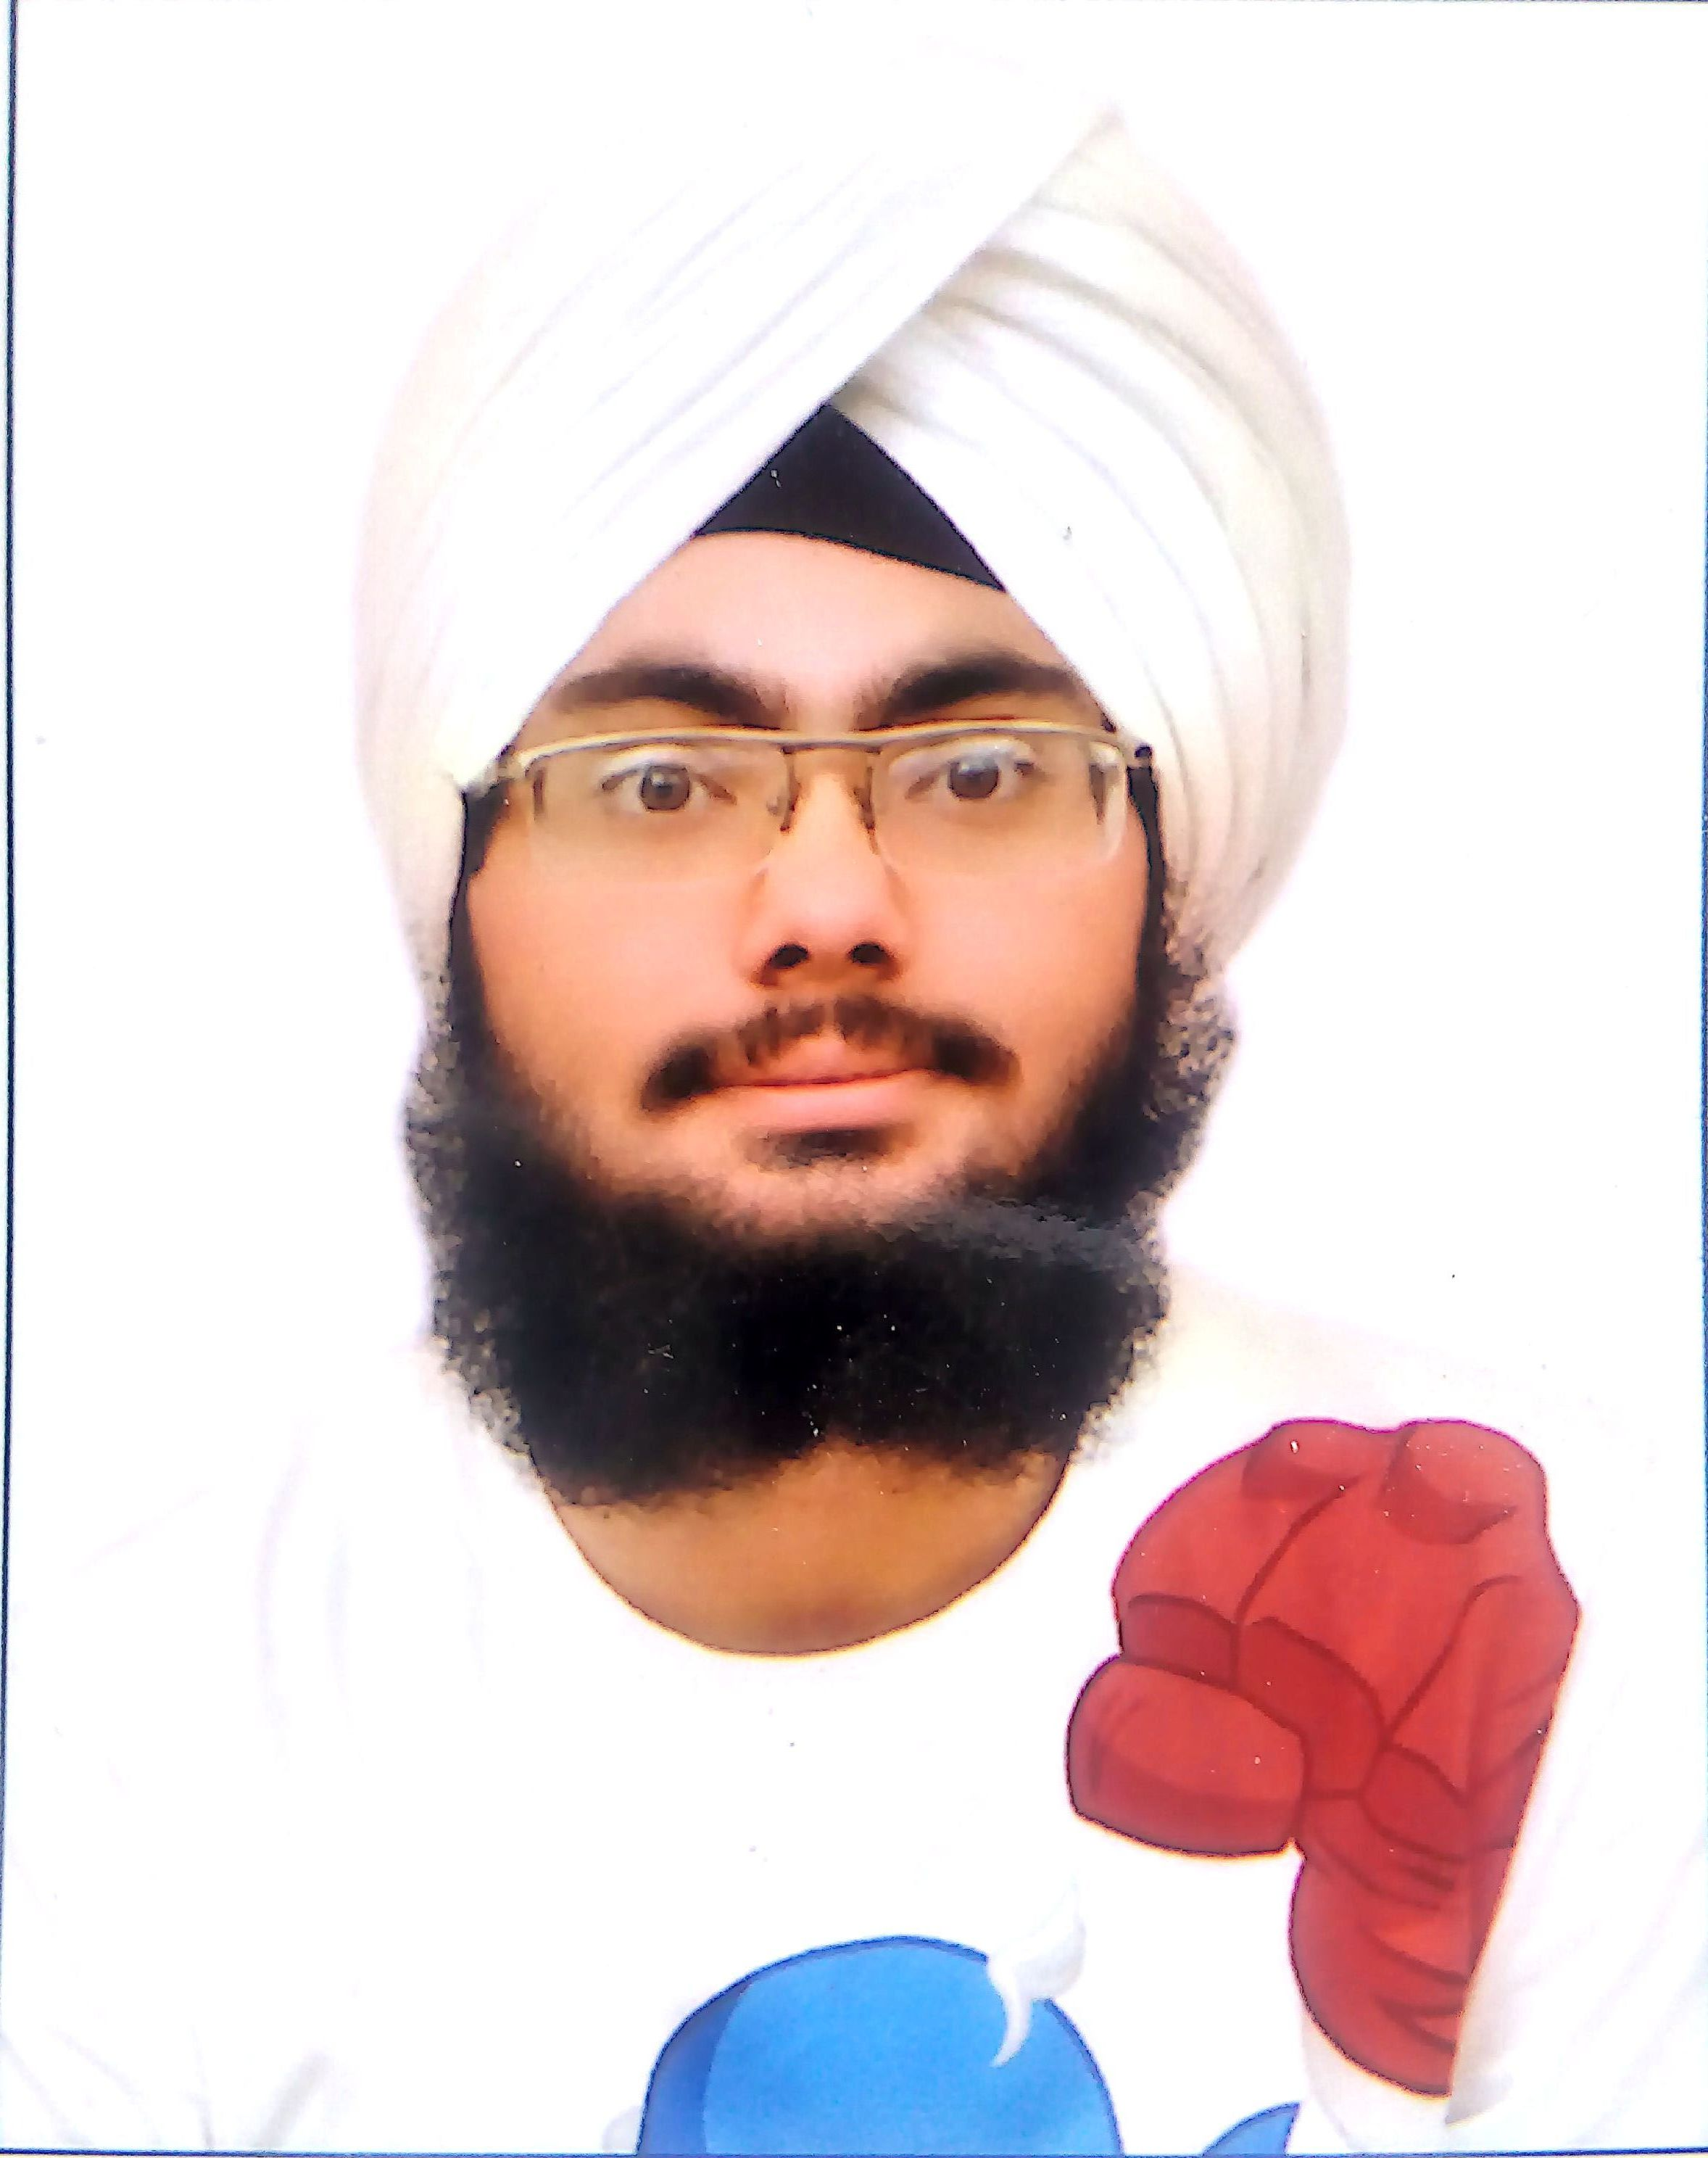
\includegraphics[width=2.5cm, height=3.5cm]{pic.jpg}	
\end{flushright}
\end{figure}



\begin{flushleft}
\textbf{OBJECTIVE }
\begin{flushright}
\vspace{-0.2in}
To develop techincal skills
\end{flushright}
\end{flushleft}



\begin{flushleft}
\vspace{0.3in}
\textbf{EDUCATION }
\begin{center}
\begin{tabular}{| L{2cm} | C{4cm} | C{2cm} | C{2cm} | R{2cm}| }
\hline
Class & School & University & Passing Year & Passing percentage\\ 
\hline
10th & APJ Public School,Sheikh Sarai,New Delhi & CBSE & 2012 & CGPA 10.0\\
\hline
12th & Ambience Public School,Safdarjung Enclave,New Delhi & CBSE & 2014 & 94.6\% \\
\hline
\end{tabular}
\end{center}
\end{flushleft}



\begin{flushleft}
\textbf{Projects }
\begin{flushright}
\begin{enumerate}
\item "Gas Leakage Detection"Theme eY-RC 16
\end{enumerate} 
\end{flushright}
\end{flushleft}



\begin{flushleft}
\textbf{Training and Internship}
\begin{flushright}
\begin{itemize}
\item Attended workshop on 8051 conducted be RoboTryst
\end{itemize} 
\end{flushright}
\end{flushleft}




\end{document}